\documentclass[11pt,a4paper]{article}

% ── Packages ──────────────────────────────────────────────
\usepackage[margin=2cm, headheight=14pt]{geometry}
\usepackage{amsmath}
\usepackage{booktabs}
\usepackage{array}
\usepackage{xcolor}
\usepackage{colortbl}
\usepackage{multirow}
\usepackage{tikz}
\usetikzlibrary{arrows.meta, patterns}
\usepackage{pgfplots}
\usepgfplotslibrary{fillbetween}
\pgfplotsset{compat=1.18}
\usepackage{siunitx}
\usepackage{enumitem}
\usepackage{fancyhdr}
\usepackage{hyperref}

% ── Colours ───────────────────────────────────────────────
\definecolor{hdrblue}{HTML}{2C3E50}
\definecolor{rowgray}{HTML}{F2F2F2}
\definecolor{accentred}{HTML}{E74C3C}
\definecolor{accentgreen}{HTML}{27AE60}
\definecolor{accentorange}{HTML}{F39C12}
\definecolor{lightblue}{HTML}{EBF5FB}

% ── Header / Footer ──────────────────────────────────────
\pagestyle{fancy}
\fancyhf{}
\lhead{\textcolor{hdrblue}{\textbf{SAFEFL --- VM Requirements}}}
\rhead{\textcolor{hdrblue}{\today}}
\cfoot{\thepage}

% ── Macros ────────────────────────────────────────────────
\newcommand{\gb}[1]{\SI{#1}{\giga\byte}}
\newcommand{\mb}[1]{\SI{#1}{\mega\byte}}
\newcommand{\sectionrule}{\noindent\textcolor{hdrblue}{\rule{\linewidth}{0.6pt}}\vspace{4pt}}

\begin{document}

% ══════════════════════════════════════════════════════════
\begin{center}
  {\LARGE\bfseries\textcolor{hdrblue}{Cloud VM Requirements}}\\[4pt]
  {\large SAFEFL Federated Learning Experimentation}\\[2pt]
  {\small Worst-case configuration\,---\,Vertex\,AI}
\end{center}
\sectionrule

% ══════════════════════════════════════════════════════════
\section*{Selected Configuration (Worst Case)}

\noindent
\begin{center}
\renewcommand{\arraystretch}{1.3}
\begin{tabular}{
  >{\raggedright\arraybackslash}p{3.8cm}
  >{\raggedright\arraybackslash}p{4.2cm}
  >{\raggedright\arraybackslash}p{6.5cm}}
\toprule
\rowcolor{hdrblue}
\textcolor{white}{\textbf{Parameter}} &
\textcolor{white}{\textbf{Selection}} &
\textcolor{white}{\textbf{Detail}} \\
\midrule
Dataset        & CIFAR-100       & $3\times32\times32$, 100 classes, 50\,k train / 10\,k test \\
\rowcolor{rowgray}
Clients        & 500             & Sequential local training per round \\
Model          & ViT-B-16        & $\sim$85.8\,M parameters ($\sim$343\,MB per gradient) \\
\rowcolor{rowgray}
Aggregation    & Krum            & $\mathcal{O}(n^{2}\!\cdot\!d)$ pairwise distance computation \\
\bottomrule
\end{tabular}
\end{center}

% ══════════════════════════════════════════════════════════
\section*{Memory Breakdown}

\noindent
\begin{center}
\renewcommand{\arraystretch}{1.3}
\begin{tabular}{
  >{\raggedright\arraybackslash}p{6.5cm}
  S[table-format=3.1]
  >{\raggedright\arraybackslash}p{4.5cm}}
\toprule
\rowcolor{hdrblue}
\textcolor{white}{\textbf{Component}} &
\textcolor{white}{\textbf{Size (GB)}} &
\textcolor{white}{\textbf{Notes}} \\
\midrule
Gradient storage ($500\times343$\,MB)
                        & 171.5 & Dominates total RAM \\
\rowcolor{rowgray}
Model + optimizer state & 1.4   & Single copy on GPU \\
Training activations    & 8.0   & Batch\,=\,32, ViT-B-16 \\
\rowcolor{rowgray}
Dataset + OS overhead   & 2.0   & CIFAR-100 + buffers \\
\midrule
\textbf{Total system RAM}    & \textbf{220.0} & \textbf{Minimum requirement} \\
\rowcolor{rowgray}
\textbf{Recommended RAM}     & \textbf{256.0} & \textbf{With safety margin} \\
\midrule
\textbf{GPU VRAM}             & \textbf{24.0}  & Single GPU sufficient \\
\bottomrule
\end{tabular}
\end{center}

% ── RAM breakdown figure ─────────────────────────────────
\noindent
\begin{center}
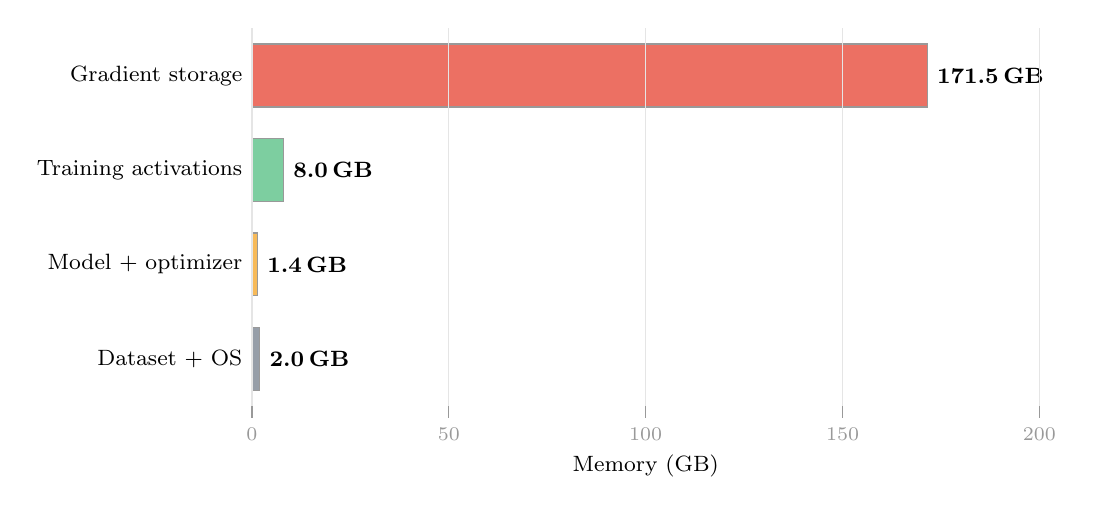
\begin{tikzpicture}
  % Manual horizontal bars using draw commands for full control
  \def\barh{0.4}  % bar half-height
  \def\yA{0}      \def\vA{2.0}    % Dataset + OS
  \def\yB{1.2}    \def\vB{1.4}    % Model + optimizer
  \def\yC{2.4}    \def\vC{8.0}    % Training activations
  \def\yD{3.6}    \def\vD{171.5}  % Gradient storage

  % Scale: 0 to 200 GB mapped to 0 to 10cm
  \def\xscale{0.05}  % 1 GB = 0.05cm → 200 GB = 10cm

  % Bars
  \fill[hdrblue!50, draw=black!40]
    (0,\yA-\barh) rectangle ({\vA*\xscale},\yA+\barh);
  \fill[accentorange!70, draw=black!40]
    (0,\yB-\barh) rectangle ({\vB*\xscale},\yB+\barh);
  \fill[accentgreen!60, draw=black!40]
    (0,\yC-\barh) rectangle ({\vC*\xscale},\yC+\barh);
  \fill[accentred!80, draw=black!40]
    (0,\yD-\barh) rectangle ({\vD*\xscale},\yD+\barh);

  % Labels on bars (right of bar end)
  \node[right, font=\footnotesize\bfseries] at ({\vA*\xscale},\yA) {2.0\,GB};
  \node[right, font=\footnotesize\bfseries] at ({\vB*\xscale},\yB) {1.4\,GB};
  \node[right, font=\footnotesize\bfseries] at ({\vC*\xscale},\yC) {8.0\,GB};
  \node[right, font=\footnotesize\bfseries] at ({\vD*\xscale},\yD) {171.5\,GB};

  % Y-axis labels
  \node[left, font=\footnotesize] at (0,\yA) {Dataset + OS};
  \node[left, font=\footnotesize] at (0,\yB) {Model + optimizer};
  \node[left, font=\footnotesize] at (0,\yC) {Training activations};
  \node[left, font=\footnotesize] at (0,\yD) {Gradient storage};

  % Axis line
  \draw[black!60] (0,-0.6) -- (0,4.2);

  % X-axis ticks
  \foreach \v/\l in {0/0, 50/50, 100/100, 150/150, 200/200} {
    \draw[black!40] ({\v*\xscale},-0.6) -- ({\v*\xscale},-0.75)
      node[below, font=\scriptsize] {\l};
    \draw[gray!20] ({\v*\xscale},-0.6) -- ({\v*\xscale},4.2);
  }
  \node[below, font=\footnotesize] at ({100*\xscale},-1.1) {Memory (GB)};

\end{tikzpicture}
\par\medskip{\small\textcolor{hdrblue}{\textbf{RAM distribution}} --- gradient storage accounts for $\sim$94\% of total memory.}
\end{center}

% ══════════════════════════════════════════════════════════
\section*{Vertex AI VM Options}

\noindent
\begin{center}
\renewcommand{\arraystretch}{1.35}
\begin{tabular}{
  >{\raggedright\arraybackslash}p{3.5cm}
  c c c
  >{\centering\arraybackslash}p{1.8cm}}
\toprule
\rowcolor{hdrblue}
\textcolor{white}{\textbf{Machine Type}} &
\textcolor{white}{\textbf{GPUs}} &
\textcolor{white}{\textbf{vCPUs}} &
\textcolor{white}{\textbf{RAM}} &
\textcolor{white}{\textbf{Verdict}} \\
\midrule
\texttt{a2-highgpu-1g}
  & 1$\times$A100\,40G & 12  & \gb{85}
  & \textcolor{accentred}{\textbf{OOM}} \\
\rowcolor{rowgray}
\texttt{a2-highgpu-2g}
  & 2$\times$A100\,40G & 24  & \gb{170}
  & \textcolor{accentorange}{\textbf{Tight}} \\
\texttt{a2-highgpu-4g}
  & 4$\times$A100\,40G & 48  & \gb{340}
  & \textcolor{accentgreen}{\textbf{Safe}} \\
\rowcolor{rowgray}
\texttt{n1-highmem-32} + A100
  & 1$\times$A100\,40G & 32  & \gb{208}
  & \textcolor{accentorange}{\textbf{Tight}} \\
\texttt{n1-highmem-64} + A100
  & 1$\times$A100\,40G & 64  & \gb{416}
  & \textcolor{accentgreen}{\textbf{Safe}} \\
\bottomrule
\end{tabular}
\end{center}

\begin{center}
\small
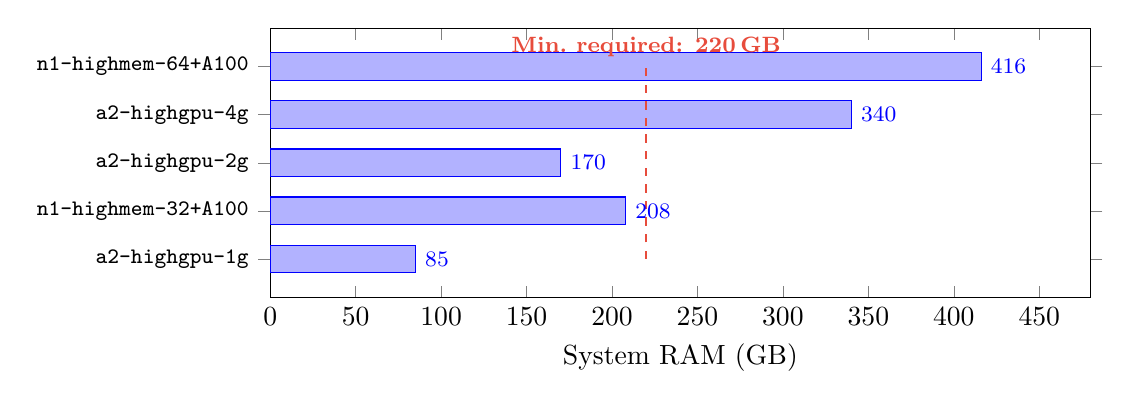
\begin{tikzpicture}
  % RAM bar chart
  \begin{axis}[
    xbar,
    width=12cm, height=5cm,
    xlabel={System RAM (GB)},
    symbolic y coords={
      {a2-highgpu-1g},
      {n1-highmem-32+A100},
      {a2-highgpu-2g},
      {a2-highgpu-4g},
      {n1-highmem-64+A100}
    },
    ytick=data,
    y tick label style={font=\ttfamily\footnotesize},
    xmin=0, xmax=480,
    bar width=10pt,
    nodes near coords,
    nodes near coords style={font=\footnotesize},
    every axis plot/.append style={fill=hdrblue!60, draw=hdrblue},
    enlarge y limits=0.2,
  ]
  \addplot coordinates {
    (85,{a2-highgpu-1g})
    (208,{n1-highmem-32+A100})
    (170,{a2-highgpu-2g})
    (340,{a2-highgpu-4g})
    (416,{n1-highmem-64+A100})
  };
  % Required line
  \draw[accentred, thick, dashed] (axis cs:220,{a2-highgpu-1g}) -- (axis cs:220,{n1-highmem-64+A100})
    node[pos=1, above, font=\footnotesize\bfseries, text=accentred] {Min.\ required: 220\,GB};
  \end{axis}
\end{tikzpicture}
\end{center}

% ══════════════════════════════════════════════════════════
\section*{Runtime Estimates (per Round, 500 Clients)}

\noindent
\begin{center}
\renewcommand{\arraystretch}{1.3}
\begin{tabular}{
  >{\raggedright\arraybackslash}p{5.5cm}
  >{\raggedright\arraybackslash}p{3.5cm}
  >{\raggedright\arraybackslash}p{5cm}}
\toprule
\rowcolor{hdrblue}
\textcolor{white}{\textbf{Phase}} &
\textcolor{white}{\textbf{Time / Round}} &
\textcolor{white}{\textbf{Complexity}} \\
\midrule
Local training (500 clients, seq.)  & 10--15\,min & $\mathcal{O}(n \cdot B \cdot d)$ \\
\rowcolor{rowgray}
Krum aggregation                    & 5--10\,min  & $\mathcal{O}(n^{2}\!\cdot\!d)$, $\sim$21.4\,T FLOPs \\
Model update + logging              & $<$1\,min   & $\mathcal{O}(d)$ \\
\midrule
\textbf{Total per round}            & \textbf{15--25\,min} & \\
\rowcolor{rowgray}
\textbf{100 rounds}                 & \textbf{25--42\,hrs} & \\
\bottomrule
\end{tabular}
\end{center}

% ══════════════════════════════════════════════════════════
\section*{Aggregation Cost Comparison at $n=500$}

\noindent
\begin{center}
\renewcommand{\arraystretch}{1.3}
\begin{tabular}{
  >{\raggedright\arraybackslash}p{3.5cm}
  >{\centering\arraybackslash}p{3.5cm}
  S[table-format=5.1]
  >{\centering\arraybackslash}p{2.2cm}}
\toprule
\rowcolor{hdrblue}
\textcolor{white}{\textbf{Method}} &
\textcolor{white}{\textbf{Complexity}} &
\textcolor{white}{\textbf{FLOPs/rnd (B)}} &
\textcolor{white}{\textbf{Relative}} \\
\midrule
FedAvg           & $\mathcal{O}(n \cdot d)$                  & 42.9    & $1\times$ \\
\rowcolor{rowgray}
Trim-Mean        & $\mathcal{O}(n \cdot d \cdot \log n)$     & 386.1   & $9\times$ \\
Median           & $\mathcal{O}(n \cdot d \cdot \log n)$     & 386.1   & $9\times$ \\
\rowcolor{rowgray}
ShieldFL / FLOD  & $\mathcal{O}(n \cdot d)$                  & 85.8    & $2\times$ \\
Divide\&Conquer  & $\mathcal{O}(t \cdot (n^{2}b + nd))$     & 2145.0  & $50\times$ \\
\rowcolor{rowgray}
\textbf{Krum}    & $\mathcal{O}(n^{2}\!\cdot\!d)$            & 21450.0 & $\mathbf{500\times}$ \\
FactorGraphs     & $\mathcal{O}(g \cdot 2^{k} + \text{BP})$  & {---}   & grouped \\
\bottomrule
\end{tabular}
\end{center}

% ── Cost scaling figure ──────────────────────────────────
\noindent
\begin{center}
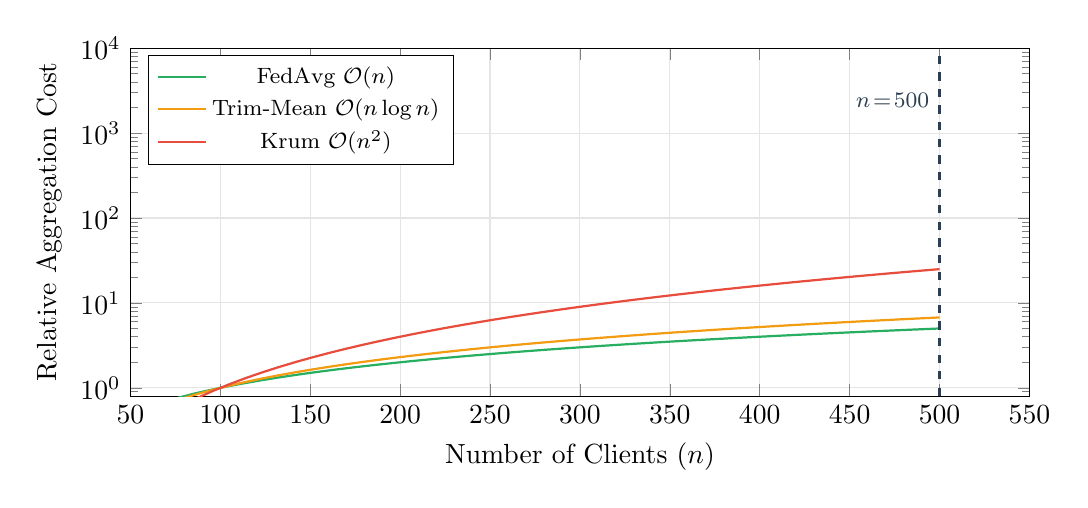
\begin{tikzpicture}
  \begin{axis}[
    width=13cm, height=6cm,
    xlabel={Number of Clients ($n$)},
    ylabel={Relative Aggregation Cost},
    ymode=log,
    xmin=50, xmax=550,
    ymin=0.8, ymax=10000,
    legend style={at={(0.02,0.98)}, anchor=north west, font=\footnotesize},
    grid=major,
    grid style={gray!20},
    every axis plot/.append style={thick},
  ]
  % FedAvg: O(n) → normalize so cost=1 at n=100
  \addplot[accentgreen, mark=none, domain=50:500, samples=50]
    {x/100};
  \addlegendentry{FedAvg $\mathcal{O}(n)$}

  % Trim-Mean: O(n log n)
  \addplot[accentorange, mark=none, domain=50:500, samples=50]
    {(x*ln(x)/ln(2)) / (100*ln(100)/ln(2))};
  \addlegendentry{Trim-Mean $\mathcal{O}(n\log n)$}

  % Krum: O(n^2)
  \addplot[accentred, mark=none, domain=50:500, samples=50]
    {(x^2) / (100^2)};
  \addlegendentry{Krum $\mathcal{O}(n^{2})$}

  % Vertical line at 500
  \draw[hdrblue, dashed, thick] (axis cs:500,0.8) -- (axis cs:500,10000)
    node[pos=0.85, left, font=\footnotesize\bfseries, text=hdrblue] {$n\!=\!500$};
  \end{axis}
\end{tikzpicture}
\par\medskip{\small\textcolor{hdrblue}{\textbf{Aggregation cost scaling}} (per-gradient-dim factor, relative to FedAvg at $n\!=\!100$).}
\end{center}

% ══════════════════════════════════════════════════════════
\section*{Recommendation}

\noindent
\begin{center}
\renewcommand{\arraystretch}{1.4}
\begin{tabular}{
  >{\raggedright\arraybackslash}p{3cm}
  >{\raggedright\arraybackslash}p{5.5cm}
  >{\raggedright\arraybackslash}p{5.5cm}}
\toprule
\rowcolor{hdrblue}
\textcolor{white}{\textbf{}} &
\textcolor{white}{\textbf{Primary (Safe)}} &
\textcolor{white}{\textbf{Budget Alternative}} \\
\midrule
Machine   & \texttt{a2-highgpu-4g}         & \texttt{n1-highmem-64} + 1$\times$A100 \\
\rowcolor{rowgray}
RAM       & \gb{340}                        & \gb{416} \\
GPU       & 4$\times$A100 40\,GB (1 used)   & 1$\times$A100 40\,GB \\
\rowcolor{rowgray}
vCPUs     & 48                              & 64 \\
Disk      & 500\,GB SSD                     & 500\,GB SSD \\
\bottomrule
\end{tabular}
\end{center}

% ══════════════════════════════════════════════════════════
\section*{Warnings}

\noindent
\begin{center}
\renewcommand{\arraystretch}{1.25}
\begin{tabular}{
  >{\centering\arraybackslash}p{0.6cm}
  >{\raggedright\arraybackslash}p{13cm}}
\toprule
\rowcolor{hdrblue}
\textcolor{white}{\textbf{\#}} &
\textcolor{white}{\textbf{Note}} \\
\midrule
1 & Gradient storage alone ($500 \times 343$\,MB $= 171.5$\,GB) will OOM any machine with $<$200\,GB RAM. \\
\rowcolor{rowgray}
2 & Krum computes $\binom{500}{2} = 124{,}750$ pairwise distances over 85.8\,M dimensions each round. \\
3 & Training is sequential (1 GPU); extra GPUs on \texttt{a2-highgpu-4g} are unused but provide the needed RAM. \\
\rowcolor{rowgray}
4 & FactorGraphs requires \texttt{group\_size} $\leq 15$ and \texttt{isGrouped=True}; cheaper than Krum at this scale. \\
\bottomrule
\end{tabular}
\end{center}

\end{document}
